%\documentclass[10pt,twocolumn,twoside]{IEEEtran}
\documentclass[journal]{IEEEtran}

% The following packages can be found on http:\\www.ctan.org
\usepackage{graphics} % for pdf, bitmapped graphics files
\usepackage{epsfig} % for postscript graphics files
\usepackage{mathptmx} % assumes new font selection scheme installed
\usepackage{times} % assumes new font selection scheme installed
\usepackage{amsmath} % assumes amsmath package installed
\usepackage{amssymb}  % assumes amsmath package installed
\usepackage{algorithm}
%\usepackage{algorithmic}
% \usepackage[utf8]{inputenc}
\usepackage[noend]{algpseudocode}
\usepackage{graphicx}
\usepackage[font=small,labelfont=bf]{caption}
\usepackage{epsfig}
\usepackage{ulem}
\usepackage{verbatim}
\usepackage{amsfonts}
\usepackage{mathrsfs}
\usepackage{breqn}
\usepackage{xcolor}
\usepackage{mathtools}
\DeclarePairedDelimiter{\ceil}{\lceil}{\rceil}
\newcommand{\qd}{\hfill{\qed}}
\def\ba{\begin{array}}
\def\ea{\end{array}}
\newcommand{\beq}{\begin{equation}}
\newcommand{\eeq}{\end{equation}}
\newcommand{\bq}{\begin{eqnarray}}
\newcommand{\eq}{\end{eqnarray}}
\newcommand{\bqn}{\begin{eqnarray*}}
\newcommand{\eqn}{\end{eqnarray*}}
\newcommand{\bee}{\begin{enumerate}}
\newcommand{\eee}{\end{enumerate}}


\RequirePackage{ifthen}
\usepackage{amssymb,mathrsfs,wasysym}
\usepackage{amsthm}
\usepackage{tikz}
\usepackage{url}
\usetikzlibrary{shadows}
\usetikzlibrary{shapes}

\newcommand{\always}{\square}
\newcommand{\eventually}{\Diamond}
\renewcommand{\next}{\ocircle}
\newcommand{\until}{\hspace{1mm}\mathcal{U}\hspace{1mm}}
\newcommand{\untilc}{\mathcal{U}}
\newcommand{\release}{\hspace{1mm}\mathcal{R}\hspace{1mm}}
\newcommand{\true}{\relax\ifmmode \mathit{True} \else \em True \/\fi}
\newcommand{\false}{\relax\ifmmode \mathit{False} \else \em False \/\fi}
\newcommand{\aand}{\hspace{1mm}\wedge\hspace{1mm}}
\newcommand{\oor}{\hspace{1mm}\vee\hspace{1mm}}
\newcommand{\set}[1]{\left\{#1\right\}}
\newcommand{\norm}[1]{\left\lVert#1\right\rVert}
\newtheorem{definition}{Definition}
\newtheorem{theorem}{Theorem}

% correct bad hyphenation here
% \hyphenation{op-tical net-works semi-conduc-tor}

\setlength{\textfloatsep}{10pt plus 1.0pt minus 2.0pt}
\begin{document}

\title{Receding Horizon Synthesis Proof}



\author{Joshua~Shaffer% <-this % stops a space
	%\thanks{J. Shaffer and H. Xu are with the Department of Aerospace Engineering,
	%	University of Maryland, College Park,
	%	MD 20740, USA e-mail: \{jshaffe9, mumu\} @umd.edu.}
	}% <-this % stops a space


% As a general rule, do not put math, special symbols or citations
% in the abstract or keywords.

\maketitle



% For peer review papers, you can put extra information on the cover
% page as needed:
% \ifCLASSOPTIONpeerreview
% \begin{center} \bfseries EDICS Category: 3-BBND \end{center}
% \fi
%
% For peerreview papers, this IEEEtran command inserts a page break and
% creates the second title. It will be ignored for other modes.
\IEEEpeerreviewmaketitle

\section{Receding Horizon Modification Proof}

%\begin{definition}
	%Left-total is defined for a set of states $s \in S$ and transitions $s \to s' \in R \subseteq S \times S$ as %$\forall s \in S$ $\exists s' \in S$ such that $s \to s' \in R$
%\end{definition}

%\begin{definition}
	%Right-total is defined for a set of states $s \in S$ and transitions $s \to s' \in R \subseteq S \times S$ as %$\forall s' \in S$ $\exists s \in S$ such that $s \to s' \in R$
%\end{definition}

\begin{definition}
	\label{definition3}
	The existence of a walk of states, composed of a finite number of subsequent transitions in $s \to s' \in T \subseteq S \times S$, such that all $s \in S$ can be eventually reached from any other initial state $s \in S$ defines the system as reachable.
\end{definition}

\begin{definition}
	\label{def2}
	The system is defined as $S = s_p \times s_o \times w$, where $s_p = \{1, 2, ...x\} \times \{1, 2, ...y\}$, $s_o = \{1, 2, 3, 4\}$, and $w = \{0, 1, 2, 3, 4\}$. $x$ and $y$ are integer values for the position in 2D space.
\end{definition}

\begin{definition}
	For all $s_{x,y} \in s_p$, $g_{x,y} = \{s \in S$ $|$ $s_{x,y} \in s\}$. In other words, $g_{x,y}$ is the set of states that contain the positional set $s_{x,y}$ that it was defined for.
\end{definition}

\begin{definition}
	\label{definition6}
	Horizons are defined for each $s_{x,y} \in s_p$ as $\mathcal{W}^{x,y}_j = \{s \in S$ $|$ $|a[1]| + |a[2]|$ $ \le 3j$ and $s \not \in \mathcal{W}^{x,y}_{j-1},$ where $a = s_{2} - s_{x,y}$ ($\forall s_2 \in s_p$) and $j > 0\}$. Furthermore, $\mathcal{W}^{x,y}_0 = g_{x,y}$. This definition is geometrically described by the horizons in Fig. \ref{WPart}
\end{definition}

\begin{definition}
	\label{definition7}
	The transition relation for the state set $S$ is defined as $T \subseteq S \times S$, where elements $s \to s' \in T$ are defined for each of the following $s'$ definitions for each $s \in S$. Note that $s' \in S$. 
	
	If $s_o \in s = 1$, $s' = \{s_{x,y} + \{0,1\},1\}$, $s' = \{s_{x,y} + \{1,1\},2\}$, and $s' = \{s_{x,y} + \{-1,1\},4\}$. 
	
	If $s_o \in s = 2$, $s' = \{s_{x,y} + \{1,0\},2\}$, $s' = \{s_{x,y} + \{1,1\},1\}$, and $s' = \{s_{x,y} + \{1,-1\},3\}$. 
	
	If $s_o \in s = 3$, $s' = \{s_{x,y} + \{0,-1\},3\}$, $s' = \{s_{x,y} + \{1,-1\},2\}$, and $s' = \{s_{x,y} + \{-1,-1\},4\}$. 
	
	If $s_o \in s = 4$, $s' = \{s_{x,y} + \{-1,0\},4\}$, $s' = \{s_{x,y} + \{-1,-1\},3\}$, and $s' = \{s_{x,y} + \{-1,1\},1\}$.
	
	This definition is geometrically described by the transitions in Fig. \ref{transitions}
\end{definition}

\begin{algorithm}
	\caption{$\mathcal{W}^{x,y}_j$ Modification during Synthesis}\label{alg:Wgen}
	\begin{algorithmic}[1]
		\Procedure{Synthesis$\_$Goal}{$x,y$}\Comment{Synthesis controllers from all initial conditions for the goal associated with location $s_{x,y}$}
		\For{$0 \le j \le N$}
		\For{$s \in \mathcal{W}_j^{x,y}$}
		\State Synthesize controller given $g_{x,y}$ and current $s$
		\If{Controller == None}
		\State Remove $s$ from $\mathcal{W}_j^{x,y}$
		\State Add $s$ to $\mathcal{W}_{j+1}^{x,y}$
		\EndIf
		\EndFor
		\EndFor
		\EndProcedure
	\end{algorithmic}
\end{algorithm}

\begin{theorem}
	Given a modified version of the system in Definition \ref{def2} which has removed some accessible states and transitions through the addition of static obstacles but still maintains the \textit{reachability} property described in Definition \ref{definition3}, and by using the initial horizons $\mathcal{W}^{x,y}_j$ described in Definition \ref{definition6} applied with the horizon modification algorithm described by Algorithm \ref{alg:Wgen}, the specification for each horizon surrounding each progress goal, $\Psi_{j}^{i}$, will remain realizable, preserving the RH framework guarantees on the overall specification.
\end{theorem}

\begin{proof}
First, we maintain that the overall specification (Eq. 3-12) is realizable for the modified system description given no horizons and any allowable initial condition. Because of such, a horizon-based synthesized solution exists that fulfills the framework and definitions provided in \cite{c10}. 

%Given the receding horizon template pictured in Fig. \ref{WPart} and formally described in Definition \ref{definition6}, guarantees regarding the satisfaction of our overall specification through the RH framework can be provided under modified horizon definitions.

%First, we only consider a subset of the total state definition that includes only location and orientation. This %is directly allowed for all horizons since specifications regarding the water levels require the position and %orientation states to reach desired goal locations $g_{i,p}$ (including the base of operations). This subset is %defined as $S_{sub} = s_p \times s_o$. We assume that a further subset of $S_{sub}$ exists (coined $S_{s}$) %such that, when combined with the transition relation defined by Definition \ref{definition7} having $S$ %replaced by $S_s$, the total state set and transition relation holds path-connectedness as defined by %Definition \ref{definition3}.

Given the Definition \ref{definition6} description of the receding horizons $\mathcal{W}^{x,y}_j$ for any individual goal $g_{x,y}$, reachability (Definition \ref{definition3}) implies that for any state sequence $\pi$ that starts and leads from $s \in \mathcal{W}^{x,y}_j$ to a state $s_f \in g_{x,y}$, said sequence $\pi$ must contain at least one $s \in \mathcal{W}^{x,y}_k$ for all $0 < k \le j$. Under the modified system definition, all available $\pi$ sequences for some $s \in \mathcal{W}^{x,y}_j$ may also need to include $s \in \mathcal{W}^{x,y}_r$ for some $r > j$, i.e. the only available path to the goal may require the state to move up horizons before moving back down due to the presence of obstacles. The possibility of such a sequence that includes paths with $s \in \mathcal{W}^{x,y}_{r > j}$ immediately violates the conditions for the receding horizon specification $\Psi_{j}^{i}$ (defined by Eq. 2). To revert this violation, modifications to the horizons are made during synthesis in order to maintain the condition that a path $\pi$ does not contain any $s \in \mathcal{W}^{x,y}_{r > j}$. This process is displayed in Algorithm \ref{alg:Wgen}.			

As controllers are synthesized around each goal and for each initial condition $s_i$ within each set $\mathcal{W}^{x,y}_j$, starting with $j = 0$ and incrementing, realizability failures are direct results of the lack of a system path to the horizon $\mathcal{W}^{x,y}_{j-1}$ that remains only in $\mathcal{W}^{x,y}_{j}$ under the assumed environment conditions. This is a result of the failure to satisfy $\Psi_{j}^{i}$ since the overall global specification is realizable. Because a path starting at the initial condition $s_i$ that fulfills the global specification must exist on the global scale and none of the sets $\mathcal{W}^{x,y}_j$ overlap per index $(x,y)$, the path must enter into $\mathcal{W}^{x,y}_{j+1}$ due to the reachability property stated before. Through the algorithm, this state $s_i$ is removed from $\mathcal{W}^{x,y}_{j}$ and added to $\mathcal{W}^{x,y}_{j+1}$. All intermediate states between the initial condition and horizon $\mathcal{W}^i_{j+1}$ are also moved to the next horizon since each state is tested as an initial condition in Algorithm \ref{alg:Wgen}, and these states cannot serve as viable initial conditions themselves. Therefore, the revised $\mathcal{W}^{x,y}_{j+1}$ contains the original set $\mathcal{W}^{x,y}_{j+1}$ plus all states from $\mathcal{W}^{x,y}_{j}$ that could not serve as initial conditions to reach the next horizon of $\mathcal{W}^{x,y}_{j-1}$ (or goal if $j-1 = 0$). This statement serves as a recursive assignment for each horizon $j$, shifting states back horizons until a new horizon set for a goal is defined such that each $s \in \mathcal{W}^{x,y}_{j}$ starts a path $\pi$ contained solely in $\mathcal{W}^{x,y}_{j}$ that reaches $\mathcal{W}^{x,y}_{j-1}$. Because of this, $\Psi_{j}^{i}$ is realizable for all goals, all horizons, and all initial conditions, maintaining the guarantees provided by the RH framework used from \cite{c10}.
\end{proof}

The benefit of the approach used by Algorithm \ref{alg:Wgen} is that the viability test for an initial condition is made during synthesis and construction of controllers, saving on computation time since the horizons aren't evaluated and modified before synthesis. Hence the original horizon definition serves as a starting point that may or may not be preserved for each goal and is only modified when necessary.

\begin{figure}
	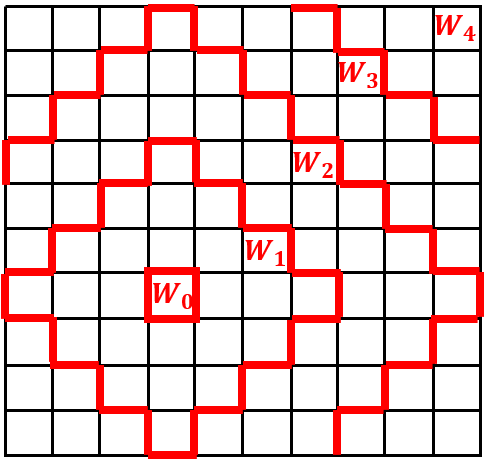
\includegraphics[width = 0.5 \linewidth]{WPartitionPic}
	\centering
	\caption{RH partitions for progress statement centered on position (4,4)}
	\label{WPart}
	\vspace*{-3mm}
\end{figure}

 \begin{figure}
	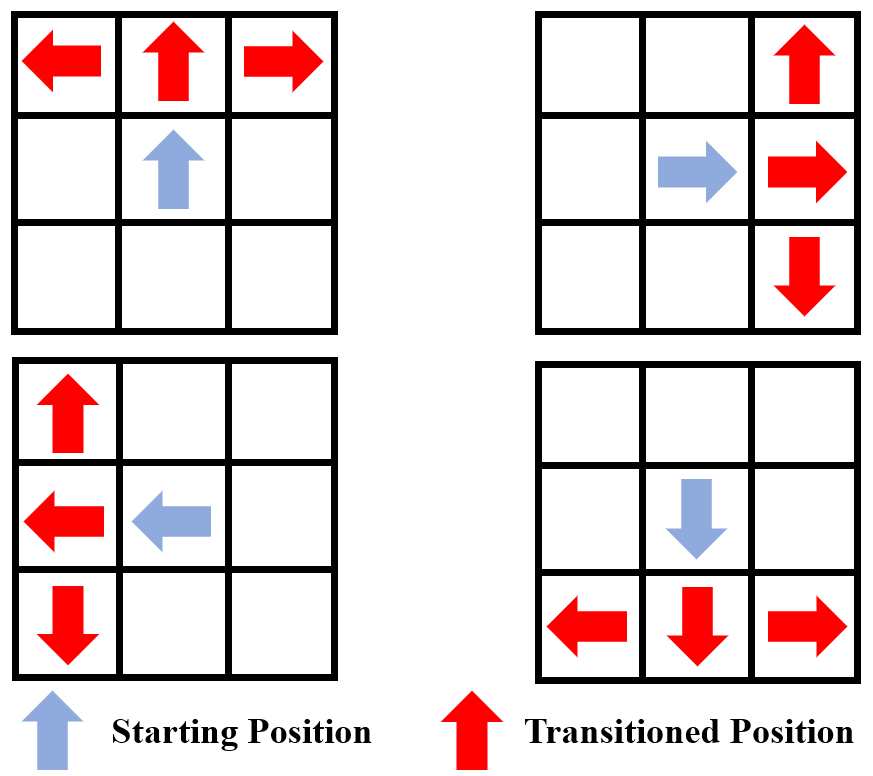
\includegraphics[width = 0.6 \linewidth]{Transitions}
	\centering
	\caption{Possible transitions for UAV within grid given starting orientation and location}
	\label{transitions}
	\vspace*{-3mm}
\end{figure}

\begin{thebibliography}{1}
	\bibitem{c10}
	T. Wongpiromsarn, U. Topcu and R. M. Murray, ``Receding Horizon Temporal Logic Planning," \textit{IEEE Transactions on Automatic Control}, vol. 57, no. 11, pp. 2817-2830, Nov. 2012.	
\end{thebibliography}

\end{document}